%! Author = Saeid Yazdani
%! Date = 4/24/2024


\section{\acs{VDUT} Concept}
\label{sec:vdut-concept}

\ac{VDUT} is a chip-package sized \ac{PCB} modeled after real \ac{DUT} that
carries the necessary circuitry and components to stimulate the ATE setup with
various load conditions as well as signal-monitoring amplifiers for
transferring the resulting waveforms to
external equipment \autocite{yazdani-vdut}.
Requirements for the \ac{VDUT} are as follows:

\begin{itemize}[topsep=8pt,itemsep=4pt,partopsep=4pt, parsep=4pt]
    \item Exact physical dimensions of the actual \ac{DUT}

    \item Able to trigger voltage rails with various types of loads:
    \begin{itemize}[topsep=8pt,itemsep=4pt,partopsep=4pt, parsep=4pt]
        \item Resistive
        \item Capacitive
        \item Inductive
    \end{itemize}

    \item Ability to capture the response on voltage rails:
    \begin{itemize}[topsep=8pt,itemsep=4pt,partopsep=4pt, parsep=4pt]
        \item Voltage waveform
        \item Current waveform
    \end{itemize}

    \item Similar electrical properties as the actual \ac{DUT} package

\end{itemize}

The general concept behind a \ac{VDUT} is to allow stimulating
\acs{ATE}'s \ac{DPS} with a precise load condition and
precise timing while monitoring the resulting voltage and current levels
exactly as it would appear on a real \ac{DUT}.

As it can be seen in \autoref{fig:vdut-in-ate-wiring-scheme}, a \ac{VDUT}
can be used as a tool to verify power supply response and signal integrity
in the total wiring scheme of the \ac{ATE} environment, including all
parasitic properties such as wiring resistance, inductance and stray
capacitance of all wires and interconnects.

\begin{figure}[htbp]
    \centering
    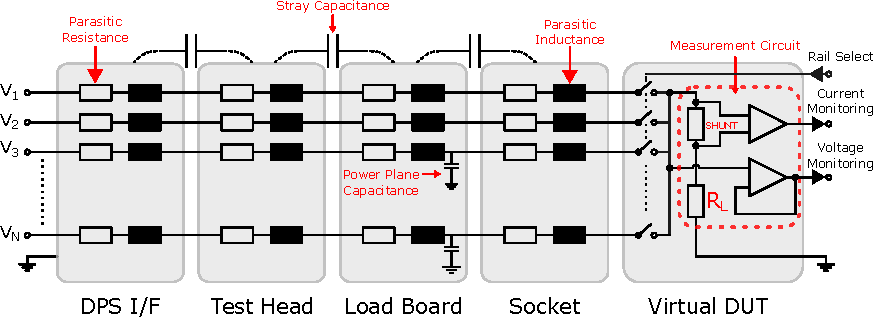
\includegraphics[width=\textwidth]
    {figures/vdut/vdut-general-concept}
    \caption[\acs{VDUT} In \ac{ATE} Wiring Scheme]{
        \ac{VDUT} Equipped with switchable loads, voltage and current
        measurement
        per supply rail or signal, allows confident measurement of
        \ac{ATE}'s \ac{DPS} unit with the total combined stray elements in the
        wiring scheme between the \ac{ATE} and \ac{DUT}.
    }
    \label{fig:vdut-in-ate-wiring-scheme}
\end{figure}

The loads on \ac{VDUT} can be triggered with precise timing using an
external controller, and the resulting voltages and currents can be
observed with external measurement equipment.
The resulting waveforms from supply rails after triggering the load(s)
will help in identifying the electrical properties of \ac{DPS}
units including response delay, rise-time, fall-time, overshoot or undershoot
and settling time.

\subsection{\acs{VDUT} Load Circuit}
\label{subsec:vdut-load-circuit}
In order to stimulate \ac{ATE}'s \ac{DPS} units using \ac{VDUT}, a known load
and a switching mechanism are available on \ac{VDUT} that switches the desired
load fully or partially on and off.

\autoref{fig:vdut-load-circuit} shows the load sub-circuit for \ac{VDUT}.
A combination of \ac{RLC} components can be switched \emph{ON} or \emph{OFF}
using a high-speed transistor controlled by an external controller's
timer unit through \ac{GPIO} pins.

\begin{figure}[h!]
    \centering
    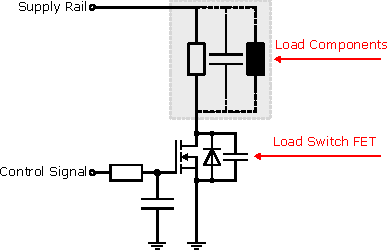
\includegraphics[width=0.80\linewidth,height=0.46\textheight,keepaspectratio]
    {figures/vdut/vdut-load-circuit}
    \caption[Load Switching Circuit of \acs{VDUT}]{
        The \ac{VDUT} can be equipped with various types of load.
        The load can be switched ON or OFF with precise timing through a
        control signal.}
    \label{fig:vdut-load-circuit}
\end{figure}

\subsection{\acs{VDUT} Measurement Circuit}
\label{subsec:vdut-measurement-circuit}
For capturing the exact response of supply rails to triggered load
condition, a buffer circuit is part of the \ac{VDUT} concept as shown in
\autoref{fig:vdut-measurement-circuit}.
To maximize power transfer and minimize signal reflections, the output of the
amplifier must be impedance-matched to the input impedance of the external
oscilloscope.
A miniature coaxial cable with \SI{50}{\ohm} characteristic impedance was
used to maintain the impedance throughout the signal path.

\begin{figure}[htbp]
    \centering
    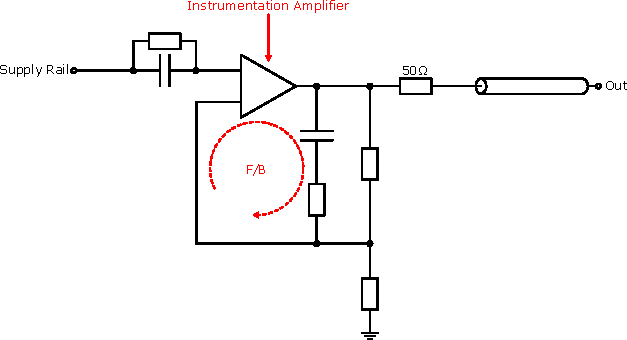
\includegraphics[width=\linewidth,height=0.62\textheight,keepaspectratio]
    {figures/vdut/vdut-measurement-circuit}
    \caption[Voltage Measurement Circuit of \acs{VDUT}]{
        A High-speed amplifier can be used to buffer and deliver the supply rail
        measurement through an impedance-matched path and coaxial connection
        to an external oscilloscope.}
    \label{fig:vdut-measurement-circuit}
\end{figure}

\subsection{\acs{VDUT} Current-Sense Circuit}
\label{subsec:vdut-current-sense-circuit}

In addition to voltage sensing, \ac{VDUT} uses a high-side current sensing
scheme to monitor the current into the triggered load as well.
\autoref{fig:vdut-current-sense-circuit} shows an amplifier configured to
use the voltage drop over a precision shunt resistor to monitor the current
supplied by \ac{DPS} units into the triggered load.


\begin{figure}[htbp]
    \centering
    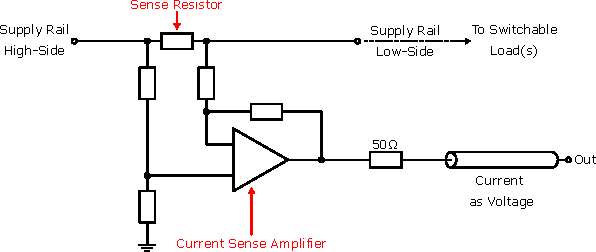
\includegraphics[width=\linewidth,height=0.62\textheight,keepaspectratio]
    {figures/vdut/vdut-current-measurement-circuit}
    \caption[Current Measurement Circuit of \acs{VDUT}]{
        High-Side current sensing arrangement to monitor the current
        of connected voltage rails.
        The voltage drop on the known precision sense resistor is translated to
        the equivalent current.
        Well-matched input resistors keep \ac{CMMR} at an acceptable amount.
    }
    \label{fig:vdut-current-sense-circuit}
\end{figure}
